\chapter{Attack Surface \& Attack Models}\label{chapter:attack-surface-models}
\todo[inline]{Improve models a lot}
Because Docker is more of an ecosystem than a single process, it has quite a large attack surface. This attack surface consists of multiple attacker models.

\medskip

In this chapter we will look at three distinct attacker models. The first two, container escapes (\autoref{subsection:container-escape}) and container-to-container attacks (\autoref{attacker-model:container-to-container-attacks}), are attacker models from inside a container. The last, Docker daemon attacks (\autoref{attacker-model:daemon-attacks}), is on a host that runs Docker.

\medskip

To clarify the attacker models, we will look at images showing each. We see the following processes pictured in the images.
\begin{enumerate}[A.]
    \item A standard (privileged) process running directly on the host.
    \item A standard unprivileged process running directly on the host.
    \item A process running in a Docker container.
    \item Similar to C.
\end{enumerate}

\section{Container Escapes}\label{subsection:container-escape}
One of the most common type of vulnerability is the possibility for a process running in a container to escape the container and access data (i.e.\ execute commands) on the host.
\begin{figure}[ht]
    \centering
    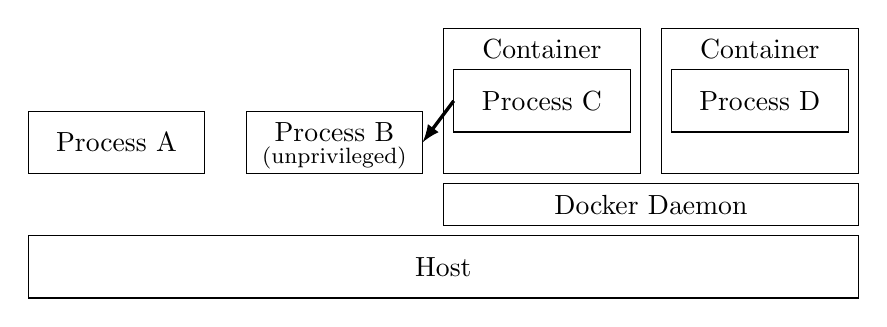
\begin{tikzpicture}[x=0.75pt,y=0.75pt,yscale=-1,xscale=1]
        % Host Rectangle
        \draw (0,100) -- (400,100) -- (400,130) -- (0,130) -- cycle ;
        \draw (200, 115) node {Host};

        %Docker Daemon Rectangle
        \draw (200,75) -- (400,75) -- (400,95) -- (200,95) -- cycle ;
        \draw (300,85) node {Docker Daemon};

        % Process A Rectangle
        \draw (0,40) -- (85,40) -- (85,70) -- (0,70) -- cycle ;
        \draw (42.5,55) node {Process A};

        % Process B Rectangle
        \draw (105,40) -- (190,40) -- (190,70) -- (105,70) -- cycle ;
        \draw (147.5,50) node {Process B};
        \draw (147.5,62.5) node {{\footnotesize (unprivileged)}};

        %Container Process C Rectangle
        \draw (200,0) -- (295,0) -- (295,70) -- (200,70) -- cycle ;
        \draw (247.5,10) node {Container};

        %% Process C Rectangle
        \draw (205,20) -- (290,20) -- (290,50) -- (205,50) -- cycle ;
        \draw (247.5,35) node {Process C};

        %Container Process D Rectangle
        \draw (305,0) -- (400,0) -- (400,70) -- (305,70) -- cycle ;
        \draw (352.5,10) node {Container};

        %% Process D Rectangle
        \draw (310,20) -- (395,20) -- (395,50) -- (310,50) -- cycle ;
        \draw (352.5,35) node {Process D};

        % Line
        \draw [latex-,very thick] (190,55) -- (205,35) ;
    \end{tikzpicture}
    \caption{}\label{fig:container-escape}
    \medskip
    \small
    A process (Process C) running inside a container accessing data on the host (that it should not be able to access), in this case Process B.
\end{figure}

\medskip

An example attack scenario would be a company that offers a Platform as a Service (PaaS) products that allows customers to run Docker containers on their infrastructure\footnote{This is actually quite common nowadays. All major computing providers offer such a service.}. If it is possible for the attacker to submit a Docker image with a malicious process that escapes the container and access the underlying infrastructure, they could access other containers or other internal resources. That would, obviously, be a very big problem for the company.

\medskip

A lot of the known container escapes are possible because the container can access some files on the host. For example, if Docker mounts some necessary directories in \lstinline{/proc} by default (which would be a vulnerability) or if sensitive data is mounted as a volume (which would be a misconfiguration).

\medskip

It be noted that an exploit that allows someone to escape from a Linux \lstinline{namespace} is essentially a container escape exploit, because Docker relies heavily on \lstinline{namespaces} for isolation (see \autoref{subsubsection:internals}). CVE--2017--7308\cite{CVE-2017-7308} is a good example of this.


\section{Container to Container Attacks}\label{attacker-model:container-to-container-attacks}
Containers should not only be isolated from the host, but also from other containers. This allows multiple containers with sensitive data to be run on the same host without them being able to access each other's data. In Docker this is not always the case.

\begin{figure}[ht]
    \centering
    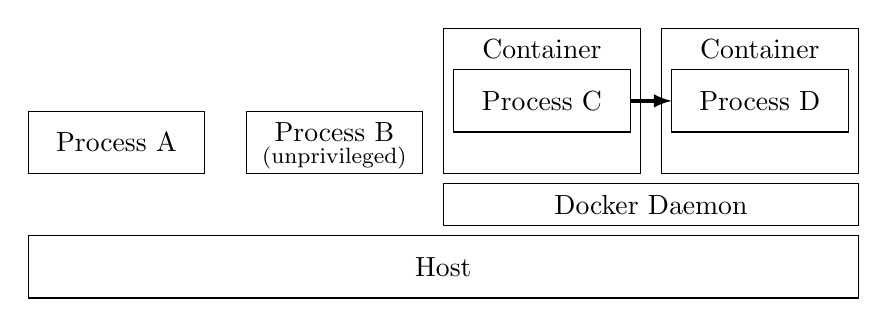
\begin{tikzpicture}[x=0.75pt,y=0.75pt,yscale=-1,xscale=1]
        % Host Rectangle
        \draw (0,100) -- (400,100) -- (400,130) -- (0,130) -- cycle ;
        \draw (200, 115) node {Host};

        %Docker Daemon Rectangle
        \draw (200,75) -- (400,75) -- (400,95) -- (200,95) -- cycle ;
        \draw (300,85) node {Docker Daemon};

        % Process A Rectangle
        \draw (0,40) -- (85,40) -- (85,70) -- (0,70) -- cycle ;
        \draw (42.5,55) node {Process A};

        % Process B Rectangle
        \draw (105,40) -- (190,40) -- (190,70) -- (105,70) -- cycle ;
        \draw (147.5,50) node {Process B};
        \draw (147.5,62.5) node {{\footnotesize (unprivileged)}};

        %Container Process C Rectangle
        \draw (200,0) -- (295,0) -- (295,70) -- (200,70) -- cycle ;
        \draw (247.5,10) node {Container};

        %% Process C Rectangle
        \draw (205,20) -- (290,20) -- (290,50) -- (205,50) -- cycle ;
        \draw (247.5,35) node {Process C};

        %Container Process D Rectangle
        \draw (305,0) -- (400,0) -- (400,70) -- (305,70) -- cycle ;
        \draw (352.5,10) node {Container};

        %% Process D Rectangle
        \draw (310,20) -- (395,20) -- (395,50) -- (310,50) -- cycle ;
        \draw (352.5,35) node {Process D};

        % Line
        \draw [-latex, very thick] (290,35) -- (310,35) ;
    \end{tikzpicture}
    \caption{}\label{fig:container-to-container-attack}
    \medskip
    \small
    A process (Process C) running inside a container, accessing data in another container (process D).
\end{figure}

By default, all Docker containers are added to the same bridge network. This means that (by default) all Docker containers can reach each other over the network. This differs from the isolation Docker uses for other \lstinline{namespaces}. In the other \lstinline{namespaces}, Docker (by default) isolates containers from the host and from other containers. This difference in design can lead to very dangerous misconfigurations, because developers may believe that Docker containers are completely isolated from each other (including the network).

\section{Docker Daemon Attack}
If user permissions are incorrectly configured, an unprivileged user can access privileged resources using the Docker daemon. This is shown in \autoref{fig:docker-daemon-attack}.

\begin{figure}[ht]
    \centering
    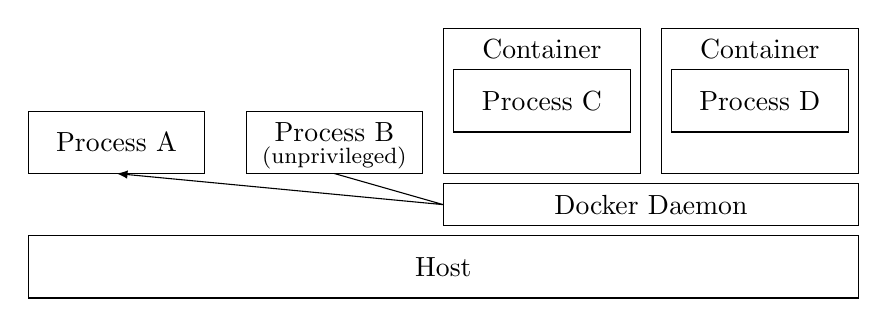
\begin{tikzpicture}[x=0.75pt,y=0.75pt,yscale=-1,xscale=1]
        % Host Rectangle
        \draw (0,100) -- (400,100) -- (400,130) -- (0,130) -- cycle ;
        \draw (200, 115) node {Host};

        %Docker Daemon Rectangle
        \draw (200,75) -- (400,75) -- (400,95) -- (200,95) -- cycle ;
        \draw (300,85) node {Docker Daemon};

        % Process A Rectangle
        \draw (0,40) -- (85,40) -- (85,70) -- (0,70) -- cycle ;
        \draw (42.5,55) node {Process A};

        % Process B Rectangle
        \draw (105,40) -- (190,40) -- (190,70) -- (105,70) -- cycle ;
        \draw (147.5,50) node {Process B};
        \draw (147.5,62.5) node {{\footnotesize (unprivileged)}};

        %Container Process C Rectangle
        \draw (200,0) -- (295,0) -- (295,70) -- (200,70) -- cycle ;
        \draw (247.5,10) node {Container};

        %% Process C Rectangle
        \draw (205,20) -- (290,20) -- (290,50) -- (205,50) -- cycle ;
        \draw (247.5,35) node {Process C};

        %Container Process D Rectangle
        \draw (305,0) -- (400,0) -- (400,70) -- (305,70) -- cycle ;
        \draw (352.5,10) node {Container};

        %% Process D Rectangle
        \draw (310,20) -- (395,20) -- (395,50) -- (310,50) -- cycle ;
        \draw (352.5,35) node {Process D};

        % Line
        \draw [-latex] (147.5,70) -- (200,85) -- (42.5,70);
    \end{tikzpicture}
    \caption{}\label{fig:docker-daemon-attack}
    \medskip
    \small
    An unprivileged process B accessing privileged data (in the image process A) using the Docker daemon.
\end{figure}

Because Docker needs a lot of kernel features to function properly, the Docker daemon needs to run as \lstinline{root}. Because Docker has many (powerful) features, this allows any user with permissions to use Docker to gain \lstinline{root} privileges. This is why the Docker documentation explicitly states ``only trusted users should be allowed to control your Docker daemon''\footnote{\url{https://docs.docker.com/engine/security/security/}}.

\medskip

A real life example of the impact of incorrectly configured Docker permissions happened a few years back with one of the courses in the Computing Science curriculum (of the Radboud). A professor wanted to teach students about containerization and modern software development. The professor asked the IT department to install Docker on all student workstations and add all the students in the course to \lstinline{docker} group (giving them full permissions to run Docker). This gave every student the equivalent of \lstinline{root} rights on every workstation. This was a problem, because it allowed students to read sensitive information (e.g.\ private keys and \lstinline{/etc/shadow}) and make changes to the system.

